%\documentclass{standalone}
%\usepackage{tikz}
%\usetikzlibrary{patterns,plotmarks}
%\begin{document}
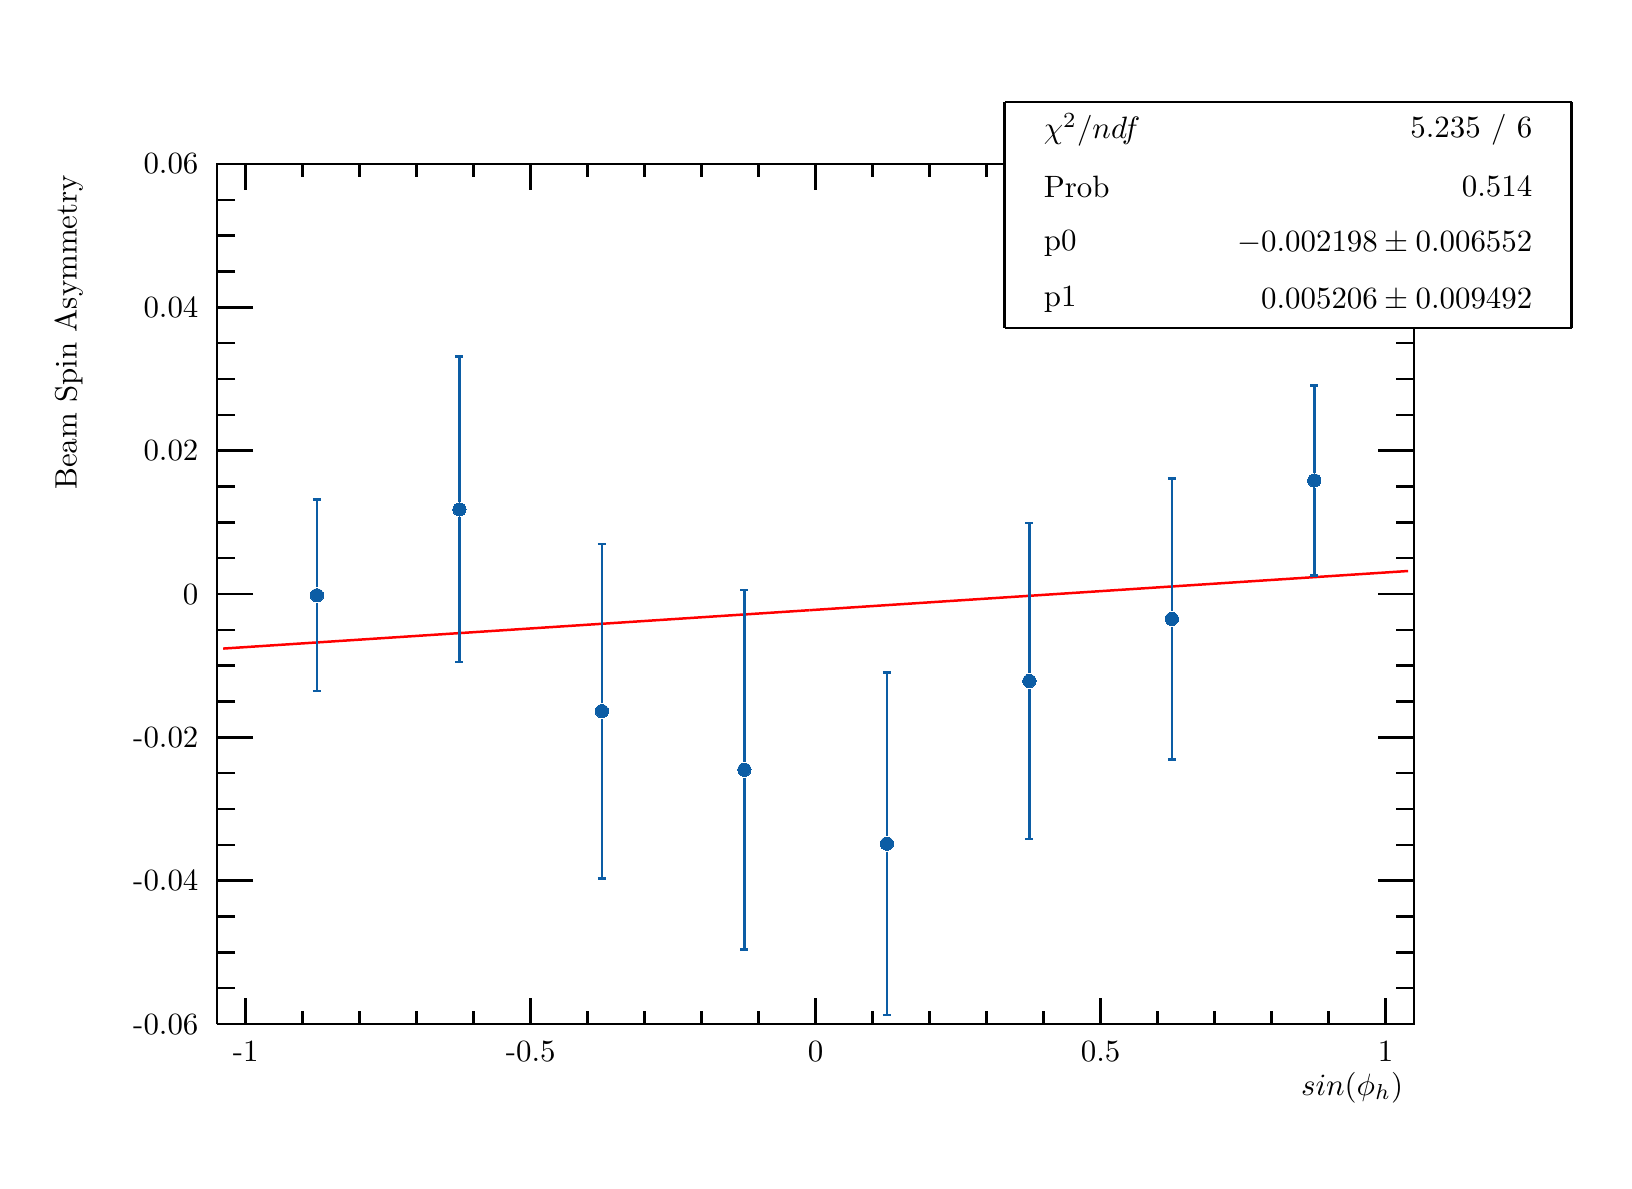
\begin{tikzpicture}
\def\CheckTikzLibraryLoaded#1{ \ifcsname tikz@library@#1@loaded\endcsname \else \PackageWarning{tikz}{usetikzlibrary{#1} is missing in the preamble.} \fi }
\CheckTikzLibraryLoaded{patterns}
\CheckTikzLibraryLoaded{plotmarks}
\pgfdeclareplotmark{cross} {
\pgfpathmoveto{\pgfpoint{-0.3\pgfplotmarksize}{\pgfplotmarksize}}
\pgfpathlineto{\pgfpoint{+0.3\pgfplotmarksize}{\pgfplotmarksize}}
\pgfpathlineto{\pgfpoint{+0.3\pgfplotmarksize}{0.3\pgfplotmarksize}}
\pgfpathlineto{\pgfpoint{+1\pgfplotmarksize}{0.3\pgfplotmarksize}}
\pgfpathlineto{\pgfpoint{+1\pgfplotmarksize}{-0.3\pgfplotmarksize}}
\pgfpathlineto{\pgfpoint{+0.3\pgfplotmarksize}{-0.3\pgfplotmarksize}}
\pgfpathlineto{\pgfpoint{+0.3\pgfplotmarksize}{-1.\pgfplotmarksize}}
\pgfpathlineto{\pgfpoint{-0.3\pgfplotmarksize}{-1.\pgfplotmarksize}}
\pgfpathlineto{\pgfpoint{-0.3\pgfplotmarksize}{-0.3\pgfplotmarksize}}
\pgfpathlineto{\pgfpoint{-1.\pgfplotmarksize}{-0.3\pgfplotmarksize}}
\pgfpathlineto{\pgfpoint{-1.\pgfplotmarksize}{0.3\pgfplotmarksize}}
\pgfpathlineto{\pgfpoint{-0.3\pgfplotmarksize}{0.3\pgfplotmarksize}}
\pgfpathclose
\pgfusepathqstroke
}
\pgfdeclareplotmark{cross*} {
\pgfpathmoveto{\pgfpoint{-0.3\pgfplotmarksize}{\pgfplotmarksize}}
\pgfpathlineto{\pgfpoint{+0.3\pgfplotmarksize}{\pgfplotmarksize}}
\pgfpathlineto{\pgfpoint{+0.3\pgfplotmarksize}{0.3\pgfplotmarksize}}
\pgfpathlineto{\pgfpoint{+1\pgfplotmarksize}{0.3\pgfplotmarksize}}
\pgfpathlineto{\pgfpoint{+1\pgfplotmarksize}{-0.3\pgfplotmarksize}}
\pgfpathlineto{\pgfpoint{+0.3\pgfplotmarksize}{-0.3\pgfplotmarksize}}
\pgfpathlineto{\pgfpoint{+0.3\pgfplotmarksize}{-1.\pgfplotmarksize}}
\pgfpathlineto{\pgfpoint{-0.3\pgfplotmarksize}{-1.\pgfplotmarksize}}
\pgfpathlineto{\pgfpoint{-0.3\pgfplotmarksize}{-0.3\pgfplotmarksize}}
\pgfpathlineto{\pgfpoint{-1.\pgfplotmarksize}{-0.3\pgfplotmarksize}}
\pgfpathlineto{\pgfpoint{-1.\pgfplotmarksize}{0.3\pgfplotmarksize}}
\pgfpathlineto{\pgfpoint{-0.3\pgfplotmarksize}{0.3\pgfplotmarksize}}
\pgfpathclose
\pgfusepathqfillstroke
}
\pgfdeclareplotmark{newstar} {
\pgfpathmoveto{\pgfqpoint{0pt}{\pgfplotmarksize}}
\pgfpathlineto{\pgfqpointpolar{44}{0.5\pgfplotmarksize}}
\pgfpathlineto{\pgfqpointpolar{18}{\pgfplotmarksize}}
\pgfpathlineto{\pgfqpointpolar{-20}{0.5\pgfplotmarksize}}
\pgfpathlineto{\pgfqpointpolar{-54}{\pgfplotmarksize}}
\pgfpathlineto{\pgfqpointpolar{-90}{0.5\pgfplotmarksize}}
\pgfpathlineto{\pgfqpointpolar{234}{\pgfplotmarksize}}
\pgfpathlineto{\pgfqpointpolar{198}{0.5\pgfplotmarksize}}
\pgfpathlineto{\pgfqpointpolar{162}{\pgfplotmarksize}}
\pgfpathlineto{\pgfqpointpolar{134}{0.5\pgfplotmarksize}}
\pgfpathclose
\pgfusepathqstroke
}
\pgfdeclareplotmark{newstar*} {
\pgfpathmoveto{\pgfqpoint{0pt}{\pgfplotmarksize}}
\pgfpathlineto{\pgfqpointpolar{44}{0.5\pgfplotmarksize}}
\pgfpathlineto{\pgfqpointpolar{18}{\pgfplotmarksize}}
\pgfpathlineto{\pgfqpointpolar{-20}{0.5\pgfplotmarksize}}
\pgfpathlineto{\pgfqpointpolar{-54}{\pgfplotmarksize}}
\pgfpathlineto{\pgfqpointpolar{-90}{0.5\pgfplotmarksize}}
\pgfpathlineto{\pgfqpointpolar{234}{\pgfplotmarksize}}
\pgfpathlineto{\pgfqpointpolar{198}{0.5\pgfplotmarksize}}
\pgfpathlineto{\pgfqpointpolar{162}{\pgfplotmarksize}}
\pgfpathlineto{\pgfqpointpolar{134}{0.5\pgfplotmarksize}}
\pgfpathclose
\pgfusepathqfillstroke
}
\definecolor{c}{rgb}{1,1,1};
\draw [color=c, fill=c] (0,0) rectangle (20,14.3719);
\draw [color=c, fill=c] (2.4,1.72462) rectangle (17.6,12.6472);
\definecolor{c}{rgb}{0,0,0};
\draw [c,line width=0.9] (2.4,1.72462) -- (2.4,12.6472) -- (17.6,12.6472) -- (17.6,1.72462) -- (2.4,1.72462);
\definecolor{c}{rgb}{1,1,1};
\draw [color=c, fill=c] (2.4,1.72462) rectangle (17.6,12.6472);
\definecolor{c}{rgb}{0,0,0};
\draw [c,line width=0.9] (2.4,1.72462) -- (2.4,12.6472) -- (17.6,12.6472) -- (17.6,1.72462) -- (2.4,1.72462);
\draw [c,line width=0.9] (2.4,1.72462) -- (17.6,1.72462);
\draw [c,line width=0.9] (2.7619,2.0523) -- (2.7619,1.72462);
\draw [c,line width=0.9] (3.48571,1.88846) -- (3.48571,1.72462);
\draw [c,line width=0.9] (4.20952,1.88846) -- (4.20952,1.72462);
\draw [c,line width=0.9] (4.93333,1.88846) -- (4.93333,1.72462);
\draw [c,line width=0.9] (5.65714,1.88846) -- (5.65714,1.72462);
\draw [c,line width=0.9] (6.38095,2.0523) -- (6.38095,1.72462);
\draw [c,line width=0.9] (7.10476,1.88846) -- (7.10476,1.72462);
\draw [c,line width=0.9] (7.82857,1.88846) -- (7.82857,1.72462);
\draw [c,line width=0.9] (8.55238,1.88846) -- (8.55238,1.72462);
\draw [c,line width=0.9] (9.27619,1.88846) -- (9.27619,1.72462);
\draw [c,line width=0.9] (10,2.0523) -- (10,1.72462);
\draw [c,line width=0.9] (10.7238,1.88846) -- (10.7238,1.72462);
\draw [c,line width=0.9] (11.4476,1.88846) -- (11.4476,1.72462);
\draw [c,line width=0.9] (12.1714,1.88846) -- (12.1714,1.72462);
\draw [c,line width=0.9] (12.8952,1.88846) -- (12.8952,1.72462);
\draw [c,line width=0.9] (13.619,2.0523) -- (13.619,1.72462);
\draw [c,line width=0.9] (14.3429,1.88846) -- (14.3429,1.72462);
\draw [c,line width=0.9] (15.0667,1.88846) -- (15.0667,1.72462);
\draw [c,line width=0.9] (15.7905,1.88846) -- (15.7905,1.72462);
\draw [c,line width=0.9] (16.5143,1.88846) -- (16.5143,1.72462);
\draw [c,line width=0.9] (17.2381,2.0523) -- (17.2381,1.72462);
\draw [c,line width=0.9] (2.7619,2.0523) -- (2.7619,1.72462);
\draw [c,line width=0.9] (17.2381,2.0523) -- (17.2381,1.72462);
\draw [anchor=base] (2.7619,1.25035) node[scale=1.11607, color=c, rotate=0]{-1};
\draw [anchor=base] (6.38095,1.25035) node[scale=1.11607, color=c, rotate=0]{-0.5};
\draw [anchor=base] (10,1.25035) node[scale=1.11607, color=c, rotate=0]{0};
\draw [anchor=base] (13.619,1.25035) node[scale=1.11607, color=c, rotate=0]{0.5};
\draw [anchor=base] (17.2381,1.25035) node[scale=1.11607, color=c, rotate=0]{1};
\draw [anchor= east] (17.6,0.919799) node[scale=1.11607, color=c, rotate=0]{$sin(\phi_{h})$};
\draw [c,line width=0.9] (2.4,12.6472) -- (17.6,12.6472);
\draw [c,line width=0.9] (2.7619,12.3196) -- (2.7619,12.6472);
\draw [c,line width=0.9] (3.48571,12.4834) -- (3.48571,12.6472);
\draw [c,line width=0.9] (4.20952,12.4834) -- (4.20952,12.6472);
\draw [c,line width=0.9] (4.93333,12.4834) -- (4.93333,12.6472);
\draw [c,line width=0.9] (5.65714,12.4834) -- (5.65714,12.6472);
\draw [c,line width=0.9] (6.38095,12.3196) -- (6.38095,12.6472);
\draw [c,line width=0.9] (7.10476,12.4834) -- (7.10476,12.6472);
\draw [c,line width=0.9] (7.82857,12.4834) -- (7.82857,12.6472);
\draw [c,line width=0.9] (8.55238,12.4834) -- (8.55238,12.6472);
\draw [c,line width=0.9] (9.27619,12.4834) -- (9.27619,12.6472);
\draw [c,line width=0.9] (10,12.3196) -- (10,12.6472);
\draw [c,line width=0.9] (10.7238,12.4834) -- (10.7238,12.6472);
\draw [c,line width=0.9] (11.4476,12.4834) -- (11.4476,12.6472);
\draw [c,line width=0.9] (12.1714,12.4834) -- (12.1714,12.6472);
\draw [c,line width=0.9] (12.8952,12.4834) -- (12.8952,12.6472);
\draw [c,line width=0.9] (13.619,12.3196) -- (13.619,12.6472);
\draw [c,line width=0.9] (14.3429,12.4834) -- (14.3429,12.6472);
\draw [c,line width=0.9] (15.0667,12.4834) -- (15.0667,12.6472);
\draw [c,line width=0.9] (15.7905,12.4834) -- (15.7905,12.6472);
\draw [c,line width=0.9] (16.5143,12.4834) -- (16.5143,12.6472);
\draw [c,line width=0.9] (17.2381,12.3196) -- (17.2381,12.6472);
\draw [c,line width=0.9] (2.7619,12.3196) -- (2.7619,12.6472);
\draw [c,line width=0.9] (17.2381,12.3196) -- (17.2381,12.6472);
\draw [c,line width=0.9] (2.4,1.72462) -- (2.4,12.6472);
\draw [c,line width=0.9] (2.856,1.72462) -- (2.4,1.72462);
\draw [c,line width=0.9] (2.628,2.17973) -- (2.4,2.17973);
\draw [c,line width=0.9] (2.628,2.63484) -- (2.4,2.63484);
\draw [c,line width=0.9] (2.628,3.08995) -- (2.4,3.08995);
\draw [c,line width=0.9] (2.856,3.54506) -- (2.4,3.54506);
\draw [c,line width=0.9] (2.628,4.00017) -- (2.4,4.00017);
\draw [c,line width=0.9] (2.628,4.45528) -- (2.4,4.45528);
\draw [c,line width=0.9] (2.628,4.91039) -- (2.4,4.91039);
\draw [c,line width=0.9] (2.856,5.36549) -- (2.4,5.36549);
\draw [c,line width=0.9] (2.628,5.8206) -- (2.4,5.8206);
\draw [c,line width=0.9] (2.628,6.27571) -- (2.4,6.27571);
\draw [c,line width=0.9] (2.628,6.73082) -- (2.4,6.73082);
\draw [c,line width=0.9] (2.856,7.18593) -- (2.4,7.18593);
\draw [c,line width=0.9] (2.628,7.64104) -- (2.4,7.64104);
\draw [c,line width=0.9] (2.628,8.09615) -- (2.4,8.09615);
\draw [c,line width=0.9] (2.628,8.55126) -- (2.4,8.55126);
\draw [c,line width=0.9] (2.856,9.00637) -- (2.4,9.00637);
\draw [c,line width=0.9] (2.628,9.46147) -- (2.4,9.46147);
\draw [c,line width=0.9] (2.628,9.91658) -- (2.4,9.91658);
\draw [c,line width=0.9] (2.628,10.3717) -- (2.4,10.3717);
\draw [c,line width=0.9] (2.856,10.8268) -- (2.4,10.8268);
\draw [c,line width=0.9] (2.628,11.2819) -- (2.4,11.2819);
\draw [c,line width=0.9] (2.628,11.737) -- (2.4,11.737);
\draw [c,line width=0.9] (2.628,12.1921) -- (2.4,12.1921);
\draw [c,line width=0.9] (2.856,12.6472) -- (2.4,12.6472);
\draw [anchor= east] (2.3,1.72462) node[scale=1.11607, color=c, rotate=0]{-0.06};
\draw [anchor= east] (2.3,3.54506) node[scale=1.11607, color=c, rotate=0]{-0.04};
\draw [anchor= east] (2.3,5.36549) node[scale=1.11607, color=c, rotate=0]{-0.02};
\draw [anchor= east] (2.3,7.18593) node[scale=1.11607, color=c, rotate=0]{0};
\draw [anchor= east] (2.3,9.00637) node[scale=1.11607, color=c, rotate=0]{0.02};
\draw [anchor= east] (2.3,10.8268) node[scale=1.11607, color=c, rotate=0]{0.04};
\draw [anchor= east] (2.3,12.6472) node[scale=1.11607, color=c, rotate=0]{0.06};
\draw [anchor= east] (0.519095,12.6472) node[scale=1.11607, color=c, rotate=90]{Beam Spin Asymmetry};
\draw [c,line width=0.9] (17.6,1.72462) -- (17.6,12.6472);
\draw [c,line width=0.9] (17.144,1.72462) -- (17.6,1.72462);
\draw [c,line width=0.9] (17.372,2.17973) -- (17.6,2.17973);
\draw [c,line width=0.9] (17.372,2.63484) -- (17.6,2.63484);
\draw [c,line width=0.9] (17.372,3.08995) -- (17.6,3.08995);
\draw [c,line width=0.9] (17.144,3.54506) -- (17.6,3.54506);
\draw [c,line width=0.9] (17.372,4.00017) -- (17.6,4.00017);
\draw [c,line width=0.9] (17.372,4.45528) -- (17.6,4.45528);
\draw [c,line width=0.9] (17.372,4.91039) -- (17.6,4.91039);
\draw [c,line width=0.9] (17.144,5.36549) -- (17.6,5.36549);
\draw [c,line width=0.9] (17.372,5.8206) -- (17.6,5.8206);
\draw [c,line width=0.9] (17.372,6.27571) -- (17.6,6.27571);
\draw [c,line width=0.9] (17.372,6.73082) -- (17.6,6.73082);
\draw [c,line width=0.9] (17.144,7.18593) -- (17.6,7.18593);
\draw [c,line width=0.9] (17.372,7.64104) -- (17.6,7.64104);
\draw [c,line width=0.9] (17.372,8.09615) -- (17.6,8.09615);
\draw [c,line width=0.9] (17.372,8.55126) -- (17.6,8.55126);
\draw [c,line width=0.9] (17.144,9.00637) -- (17.6,9.00637);
\draw [c,line width=0.9] (17.372,9.46147) -- (17.6,9.46147);
\draw [c,line width=0.9] (17.372,9.91658) -- (17.6,9.91658);
\draw [c,line width=0.9] (17.372,10.3717) -- (17.6,10.3717);
\draw [c,line width=0.9] (17.144,10.8268) -- (17.6,10.8268);
\draw [c,line width=0.9] (17.372,11.2819) -- (17.6,11.2819);
\draw [c,line width=0.9] (17.372,11.737) -- (17.6,11.737);
\draw [c,line width=0.9] (17.372,12.1921) -- (17.6,12.1921);
\draw [c,line width=0.9] (17.144,12.6472) -- (17.6,12.6472);
\definecolor{c}{rgb}{0.0470588,0.364706,0.647059};
\foreach \P in {(3.66667,7.16966), (5.47619,8.26066), (7.28571,5.69865), (9.09524,4.95472), (10.9048,4.01498), (12.7143,6.08183), (14.5238,6.87073), (16.3333,8.62818)}{\draw[mark options={color=c,fill=c},mark size=2.402402pt, line width=0.000000pt,
 mark=*] plot coordinates {\P};}
\definecolor{c}{rgb}{1,0,0};
\draw [c,line width=0.9] (2.476,6.49336) -- (2.628,6.50331) -- (2.78,6.51326) -- (2.932,6.52321) -- (3.084,6.53316) -- (3.236,6.54311) -- (3.388,6.55306) -- (3.54,6.56301) -- (3.692,6.57296) -- (3.844,6.58291) -- (3.996,6.59286) -- (4.148,6.60281) --
 (4.3,6.61276) -- (4.452,6.62271) -- (4.604,6.63267) -- (4.756,6.64262) -- (4.908,6.65257) -- (5.06,6.66252) -- (5.212,6.67247) -- (5.364,6.68242) -- (5.516,6.69237) -- (5.668,6.70232) -- (5.82,6.71227) -- (5.972,6.72222) -- (6.124,6.73217) --
 (6.276,6.74212) -- (6.428,6.75207) -- (6.58,6.76202) -- (6.732,6.77197) -- (6.884,6.78192) -- (7.036,6.79187) -- (7.188,6.80182) -- (7.34,6.81177) -- (7.492,6.82172) -- (7.644,6.83167) -- (7.796,6.84162) -- (7.948,6.85157) -- (8.1,6.86153) --
 (8.252,6.87148) -- (8.404,6.88143) -- (8.556,6.89138) -- (8.708,6.90133) -- (8.86,6.91128) -- (9.012,6.92123) -- (9.164,6.93118) -- (9.316,6.94113) -- (9.468,6.95108) -- (9.62,6.96103) -- (9.772,6.97098) -- (9.924,6.98093);
\draw [c,line width=0.9] (9.924,6.98093) -- (10.076,6.99088) -- (10.228,7.00083) -- (10.38,7.01078) -- (10.532,7.02073) -- (10.684,7.03068) -- (10.836,7.04063) -- (10.988,7.05058) -- (11.14,7.06053) -- (11.292,7.07048) -- (11.444,7.08043) --
 (11.596,7.09038) -- (11.748,7.10034) -- (11.9,7.11029) -- (12.052,7.12024) -- (12.204,7.13019) -- (12.356,7.14014) -- (12.508,7.15009) -- (12.66,7.16004) -- (12.812,7.16999) -- (12.964,7.17994) -- (13.116,7.18989) -- (13.268,7.19984) --
 (13.42,7.20979) -- (13.572,7.21974) -- (13.724,7.22969) -- (13.876,7.23964) -- (14.028,7.24959) -- (14.18,7.25954) -- (14.332,7.26949) -- (14.484,7.27944) -- (14.636,7.28939) -- (14.788,7.29934) -- (14.94,7.30929) -- (15.092,7.31924) --
 (15.244,7.3292) -- (15.396,7.33915) -- (15.548,7.3491) -- (15.7,7.35905) -- (15.852,7.369) -- (16.004,7.37895) -- (16.156,7.3889) -- (16.308,7.39885) -- (16.46,7.4088) -- (16.612,7.41875) -- (16.764,7.4287) -- (16.916,7.43865) -- (17.068,7.4486) --
 (17.22,7.45855) -- (17.372,7.4685);
\draw [c,line width=0.9] (17.372,7.4685) -- (17.524,7.47845);
\definecolor{c}{rgb}{1,1,1};
\draw [color=c, fill=c] (12.4,10.5633) rectangle (19.6,13.4377);
\definecolor{c}{rgb}{0,0,0};
\draw [c,line width=0.9] (12.4,10.5633) -- (19.6,10.5633);
\draw [c,line width=0.9] (19.6,10.5633) -- (19.6,13.4377);
\draw [c,line width=0.9] (19.6,13.4377) -- (12.4,13.4377);
\draw [c,line width=0.9] (12.4,13.4377) -- (12.4,10.5633);
\draw [anchor= west] (12.76,13.0784) node[scale=1.11607, color=c, rotate=0]{$\chi^{2} / ndf $};
\draw [anchor= east] (19.24,13.0784) node[scale=1.11607, color=c, rotate=0]{ 5.235 / 6};
\draw [anchor= west] (12.76,12.3598) node[scale=1.11607, color=c, rotate=0]{Prob  };
\draw [anchor= east] (19.24,12.3598) node[scale=1.11607, color=c, rotate=0]{ 0.514};
\draw [anchor= west] (12.76,11.6412) node[scale=1.11607, color=c, rotate=0]{p0       };
\draw [anchor= east] (19.24,11.6412) node[scale=1.11607, color=c, rotate=0]{$ -0.002198 \pm 0.006552$};
\draw [anchor= west] (12.76,10.9226) node[scale=1.11607, color=c, rotate=0]{p1       };
\draw [anchor= east] (19.24,10.9226) node[scale=1.11607, color=c, rotate=0]{$ 0.005206 \pm 0.009492$};
\definecolor{c}{rgb}{0.0470588,0.364706,0.647059};
\draw [c,line width=0.9] (3.66667,7.27016) -- (3.66667,8.38675);
\draw [c,line width=0.9] (3.66667,7.06915) -- (3.66667,5.95257);
\draw [c,line width=0.9] (3.61642,8.38675) -- (3.71692,8.38675);
\draw [c,line width=0.9] (3.61642,5.95257) -- (3.71692,5.95257);
\draw [c,line width=0.9] (5.47619,8.36117) -- (5.47619,10.2004);
\draw [c,line width=0.9] (5.47619,8.16016) -- (5.47619,6.32096);
\draw [c,line width=0.9] (5.42594,10.2004) -- (5.52644,10.2004);
\draw [c,line width=0.9] (5.42594,6.32096) -- (5.52644,6.32096);
\draw [c,line width=0.9] (7.28571,5.79915) -- (7.28571,7.82291);
\draw [c,line width=0.9] (7.28571,5.59814) -- (7.28571,3.57438);
\draw [c,line width=0.9] (7.23546,7.82291) -- (7.33597,7.82291);
\draw [c,line width=0.9] (7.23546,3.57438) -- (7.33597,3.57438);
\draw [c,line width=0.9] (9.09524,5.05523) -- (9.09524,7.23669);
\draw [c,line width=0.9] (9.09524,4.85422) -- (9.09524,2.67275);
\draw [c,line width=0.9] (9.04499,7.23669) -- (9.14549,7.23669);
\draw [c,line width=0.9] (9.04499,2.67275) -- (9.14549,2.67275);
\draw [c,line width=0.9] (10.9048,4.11549) -- (10.9048,6.1902);
\draw [c,line width=0.9] (10.9048,3.91448) -- (10.9048,1.83977);
\draw [c,line width=0.9] (10.8545,6.1902) -- (10.955,6.1902);
\draw [c,line width=0.9] (10.8545,1.83977) -- (10.955,1.83977);
\draw [c,line width=0.9] (12.7143,6.18233) -- (12.7143,8.08679);
\draw [c,line width=0.9] (12.7143,5.98133) -- (12.7143,4.07687);
\draw [c,line width=0.9] (12.664,8.08679) -- (12.7645,8.08679);
\draw [c,line width=0.9] (12.664,4.07687) -- (12.7645,4.07687);
\draw [c,line width=0.9] (14.5238,6.97124) -- (14.5238,8.65616);
\draw [c,line width=0.9] (14.5238,6.77023) -- (14.5238,5.08531);
\draw [c,line width=0.9] (14.4736,8.65616) -- (14.5741,8.65616);
\draw [c,line width=0.9] (14.4736,5.08531) -- (14.5741,5.08531);
\draw [c,line width=0.9] (16.3333,8.72868) -- (16.3333,9.83591);
\draw [c,line width=0.9] (16.3333,8.52767) -- (16.3333,7.42044);
\draw [c,line width=0.9] (16.2831,9.83591) -- (16.3836,9.83591);
\draw [c,line width=0.9] (16.2831,7.42044) -- (16.3836,7.42044);
\definecolor{c}{rgb}{1,1,1};
\draw [color=c, fill=c] (12.4,10.5633) rectangle (19.6,13.4377);
\definecolor{c}{rgb}{0,0,0};
\draw [c,line width=0.9] (12.4,10.5633) -- (19.6,10.5633);
\draw [c,line width=0.9] (19.6,10.5633) -- (19.6,13.4377);
\draw [c,line width=0.9] (19.6,13.4377) -- (12.4,13.4377);
\draw [c,line width=0.9] (12.4,13.4377) -- (12.4,10.5633);
\draw [anchor= west] (12.76,13.0784) node[scale=1.11607, color=c, rotate=0]{$\chi^{2} / ndf $};
\draw [anchor= east] (19.24,13.0784) node[scale=1.11607, color=c, rotate=0]{ 5.235 / 6};
\draw [anchor= west] (12.76,12.3598) node[scale=1.11607, color=c, rotate=0]{Prob  };
\draw [anchor= east] (19.24,12.3598) node[scale=1.11607, color=c, rotate=0]{ 0.514};
\draw [anchor= west] (12.76,11.6412) node[scale=1.11607, color=c, rotate=0]{p0       };
\draw [anchor= east] (19.24,11.6412) node[scale=1.11607, color=c, rotate=0]{$ -0.002198 \pm 0.006552$};
\draw [anchor= west] (12.76,10.9226) node[scale=1.11607, color=c, rotate=0]{p1       };
\draw [anchor= east] (19.24,10.9226) node[scale=1.11607, color=c, rotate=0]{$ 0.005206 \pm 0.009492$};
\end{tikzpicture}
%\end{document}
